\section{Projektowanie powiązań (relacji) pomiędzy encjami}

% \textit{Konstrukcja diagramu ERD
% (Entity-Relationship Diagram); jest to zasadniczy etap procesu projektowania struktury
% bazy danych. Identyfikacja klas encji, ich atrybutów, zdefiniowanie (określenie) kluczy.
% Tablica krzyżowa powiązań, eliminacja powiązań wiele-do-wielu. Konstrukcja diagramu
% ERD.} \\

Diagram ERD przedstawiono na rysunku \ref{fig:erd}.

\begin{figure}[!htp]
    \centering
    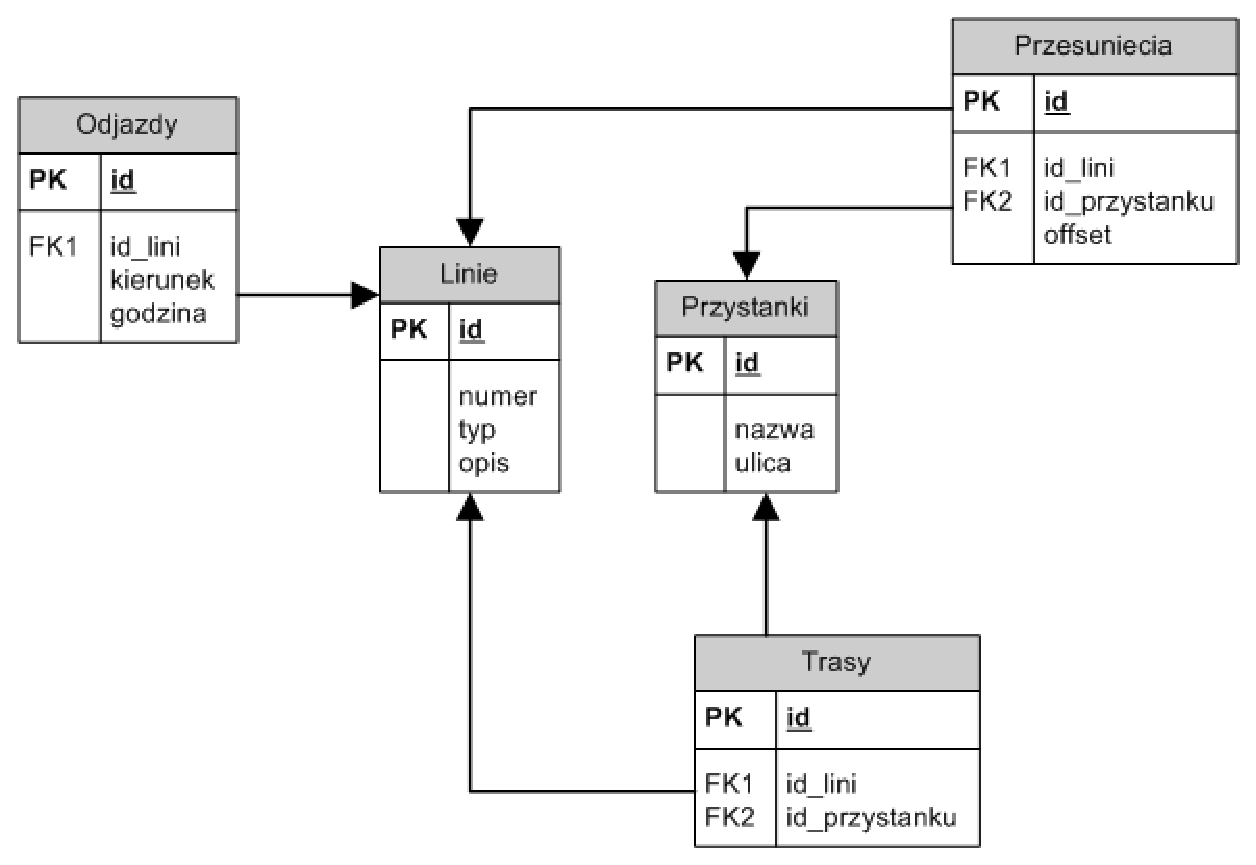
\includegraphics[width=0.4\textwidth]{./img/bus-agenda-erd.eps}
    \caption{Diagram ERD}
    \label{fig:erd}
\end{figure}

